% Generated by recon/fig-filtration.mjs — do not edit by hand.
% Regenerate after any change to ring-domain / ring-objective / ring-evidence.
\documentclass[tikz,border=3pt]{standalone}
\usepackage{pgfplots}
\pgfplotsset{compat=1.18}
\usepgfplotslibrary{groupplots}
\usepackage{amsmath}

\definecolor{Guidocol}{HTML}{2a78d6}
\definecolor{Pompiliacol}{HTML}{eb6834}
\definecolor{Caponsacchicol}{HTML}{1baf7a}
\definecolor{feascol}{HTML}{52514E}
\definecolor{inkcol}{HTML}{0B0B0B}

\begin{document}
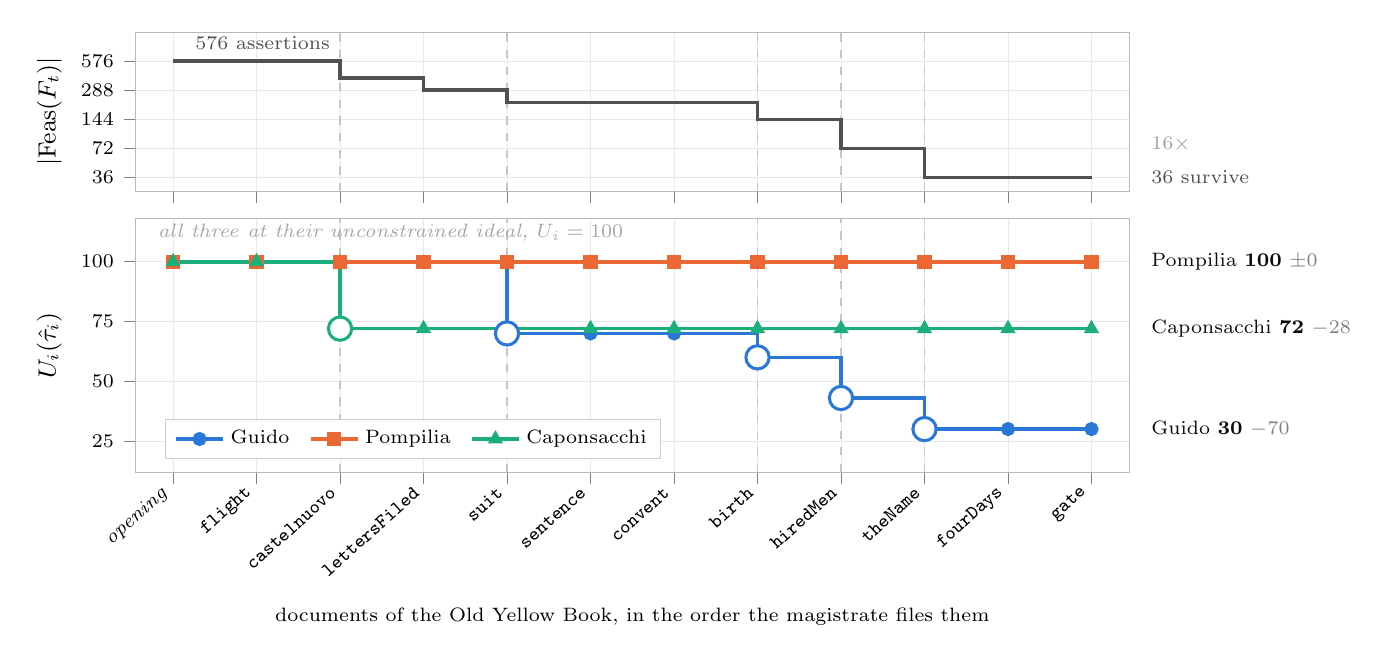
\begin{tikzpicture}[font=\small]
\begin{groupplot}[
    group style={group size=1 by 2, vertical sep=3.5mm, x descriptions at=edge bottom},
    width=14.2cm,
    xmin=-0.45, xmax=11.45,
    xtick={0,1,2,3,4,5,6,7,8,9,10,11},
    xticklabels={\textit{opening}, \texttt{flight}, \texttt{castelnuovo}, \texttt{lettersFiled}, \texttt{suit}, \texttt{sentence}, \texttt{convent}, \texttt{birth}, \texttt{hiredMen}, \texttt{theName}, \texttt{fourDays}, \texttt{gate}},
    x tick label style={rotate=42, anchor=east, font=\scriptsize},
    tick align=outside, tick pos=left,
    axis line style={gray!55, line width=0.4pt},
    grid=major, grid style={gray!18, line width=0.3pt},
    every axis plot/.append style={line width=1.3pt},
    label style={font=\small}, tick label style={font=\scriptsize},
  ]

  %% ---- top panel: the filtration itself ----
  \nextgroupplot[
    height=3.6cm, ymode=log, ymin=26, ymax=1150, clip=false,
    ytick={36,72,144,288,576}, yticklabels={36,72,144,288,576},
    log ticks with fixed point,
    ylabel={$|\mathrm{Feas}(F_t)|$},
    ylabel style={align=center},
  ]
    \draw[gray!45, dashed, line width=0.4pt] (axis cs:2,26) -- (axis cs:2,1150);
    \draw[gray!45, dashed, line width=0.4pt] (axis cs:4,26) -- (axis cs:4,1150);
    \draw[gray!45, dashed, line width=0.4pt] (axis cs:7,26) -- (axis cs:7,1150);
    \draw[gray!45, dashed, line width=0.4pt] (axis cs:8,26) -- (axis cs:8,1150);
    \draw[gray!45, dashed, line width=0.4pt] (axis cs:9,26) -- (axis cs:9,1150);
    \addplot[const plot, mark=none, color=feascol] coordinates {(0,576) (1,576) (2,384) (3,288) (4,216) (5,216) (6,216) (7,144) (8,72) (9,36) (10,36) (11,36)};
    \node[anchor=west, font=\scriptsize, text=feascol] at (axis cs:0.15,880) {576 assertions};
    \node[anchor=west, font=\scriptsize, text=feascol] at (axis cs:11.6,36) {36 survive};
    \node[anchor=west, font=\scriptsize\itshape, text=gray!75] at (axis cs:11.6,80) {$16\times$};

  %% ---- bottom panel: what it cost each witness ----
  \nextgroupplot[
    height=4.8cm, ymin=12, ymax=118, clip=false,
    ytick={25,50,75,100},
    ylabel={$U_i(\hat\tau_i)$},
    xlabel={documents of the Old Yellow Book, in the order the magistrate files them},
    xlabel style={font=\scriptsize, yshift=-1mm},
    legend style={at={(0.03,0.05)}, anchor=south west, draw=gray!40, fill=white,
                  font=\scriptsize, row sep=-1pt, /tikz/every even column/.append style={column sep=5pt}},
    legend columns=3,
  ]
    \draw[gray!45, dashed, line width=0.4pt] (axis cs:2,12) -- (axis cs:2,118);
    \draw[gray!45, dashed, line width=0.4pt] (axis cs:4,12) -- (axis cs:4,118);
    \draw[gray!45, dashed, line width=0.4pt] (axis cs:7,12) -- (axis cs:7,118);
    \draw[gray!45, dashed, line width=0.4pt] (axis cs:8,12) -- (axis cs:8,118);
    \draw[gray!45, dashed, line width=0.4pt] (axis cs:9,12) -- (axis cs:9,118);
    \addplot[const plot, mark=*, mark size=1.9pt, color=Guidocol] coordinates {(0,100) (1,100) (2,100) (3,100) (4,70) (5,70) (6,70) (7,60) (8,43) (9,30) (10,30) (11,30)};
    \addlegendentry{Guido}
    \addplot[const plot, mark=square*, mark size=1.9pt, color=Pompiliacol] coordinates {(0,100) (1,100) (2,100) (3,100) (4,100) (5,100) (6,100) (7,100) (8,100) (9,100) (10,100) (11,100)};
    \addlegendentry{Pompilia}
    \addplot[const plot, mark=triangle*, mark size=1.9pt, color=Caponsacchicol] coordinates {(0,100) (1,100) (2,72) (3,72) (4,72) (5,72) (6,72) (7,72) (8,72) (9,72) (10,72) (11,72)};
    \addlegendentry{Caponsacchi}
    \addplot[only marks, mark=*, mark size=4.2pt, draw=Guidocol, fill=white, line width=1.1pt, forget plot]
      coordinates {(4,70) (7,60) (8,43) (9,30)};
    \addplot[only marks, mark=*, mark size=4.2pt, draw=Caponsacchicol, fill=white, line width=1.1pt, forget plot]
      coordinates {(2,72)};
    \node[anchor=west, font=\scriptsize, text=inkcol] at (axis cs:11.6,30) {Guido\ \textbf{30}\ \textcolor{gray}{\textit{$-70$}}};
    \node[anchor=west, font=\scriptsize, text=inkcol] at (axis cs:11.6,100) {Pompilia\ \textbf{100}\ \textcolor{gray}{\textit{$\pm0$}}};
    \node[anchor=west, font=\scriptsize, text=inkcol] at (axis cs:11.6,72) {Caponsacchi\ \textbf{72}\ \textcolor{gray}{\textit{$-28$}}};
    \node[anchor=west, font=\scriptsize\itshape, text=gray!70] at (axis cs:-0.3,112) {all three at their unconstrained ideal, $U_i=100$};

\end{groupplot}
\end{tikzpicture}
\end{document}
